\chapter{Estados}
\section{Introduccion}
\begin{flushleft}
	
El diagrama de estado se usa para dar forma al comportamiento de un objeto, de una clase. Se representa la secuencia de estados que un objeto de la clase tiene durante su vida, según las acciones que van sucediendo.
\\
Las características de los diagramas de estados se puede resumir en estas tres:\\
 - Un estado es la representación de un objeto en los diferentes espacios de tiempo que le van sucediendo. Cuando hablamos de estado estamos hablando de los diferentes estados que puede tener un objeto.\\
 - Cada evento representa algo que hace que nuestro objeto pueda cambiar.\\
 - Existen unas líneas que llamamos líneas de transición, su finalidad es describir el movimiento de un estado a otro. A estas líneas le ponemos el nombre del evento que origina la transición.
\end{flushleft}
\newpage
\section{Diagrama de Estados}
\begin{flushleft}
A continuacion, esta la ejemplificacion de un diagrama de estados aplicado a nuestro proyecto de parqueos, donde se van alterando los distintos estados de un parqueo, que puede tener unicamente tres estados en concreto, el estado base de un parqueadero es el estado "Disponible", que indica que el espacio de parqueo es apto para ser ocupado por un vehiculo de un tipo particular, es decir, el espacio puede ser tomado en alquiler por un usuario. Un segundo estado que es el de "Ocupado", le señala al usuario que el espacio de parqueo no puede ser tomado en uso por un tiempo determinado. Y, por ultimo, esta el estado "Invisible", que señala que un parqueadero no esta ni Disponible, ni Ocupado, simplemente el dueño de este espacio decide no mostrarlo como espacio seleccionable, por lo que sus datos tampoco son visibles al resto de usuarios, en otras palabras, el dueño puede ocultar su parqueadero si simplemente no quiere alquilarlo por un tiempo.
\\
A continuación esta el diagrama de estados de nuestro proyecto de parqueos, donde, como se menciono anteriormente, solo se incluyen 3 estados, que corresponde a cualquier tipo de espacio de parqueo:
\\
\begin{center}
{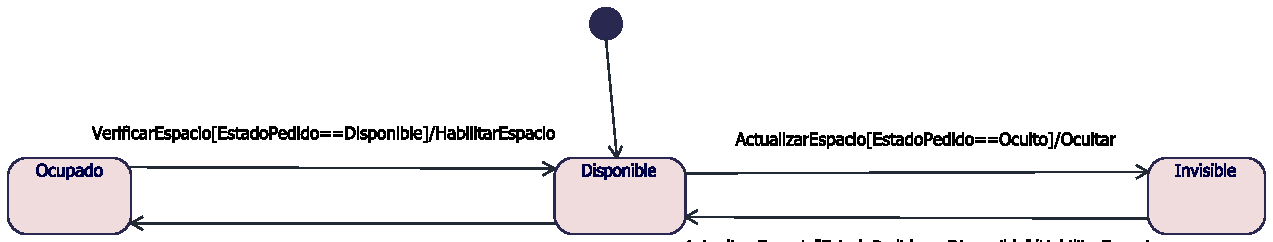
\includegraphics[width=1.18\linewidth]{imgs/Imagenes - Diagrama de estados/Estados}}
\end{center}

\end{flushleft}
\newpage
\subsection{Diagrama de Clase}
\begin{flushleft}
Tanto el diagrama anterior, como los siguientes, fueron elaborados gracias a la herramienta de diseño Coloso, la cual, al momento de construir el diagrama de estados con su respectivo Disparador (Metodo que da accion al cambio de estados), condicional (sentencia que se tiene que cumplir para efectuar el cambio) y efecto (metodo que realiza el cambio de estado como tal). La herramienta coloso ademas de construir el diagrama de estados con estos elementos, genera un diagrama de clase con los metodos y atributos correspondientes a dicho diagrama:
\\
\begin{center}
{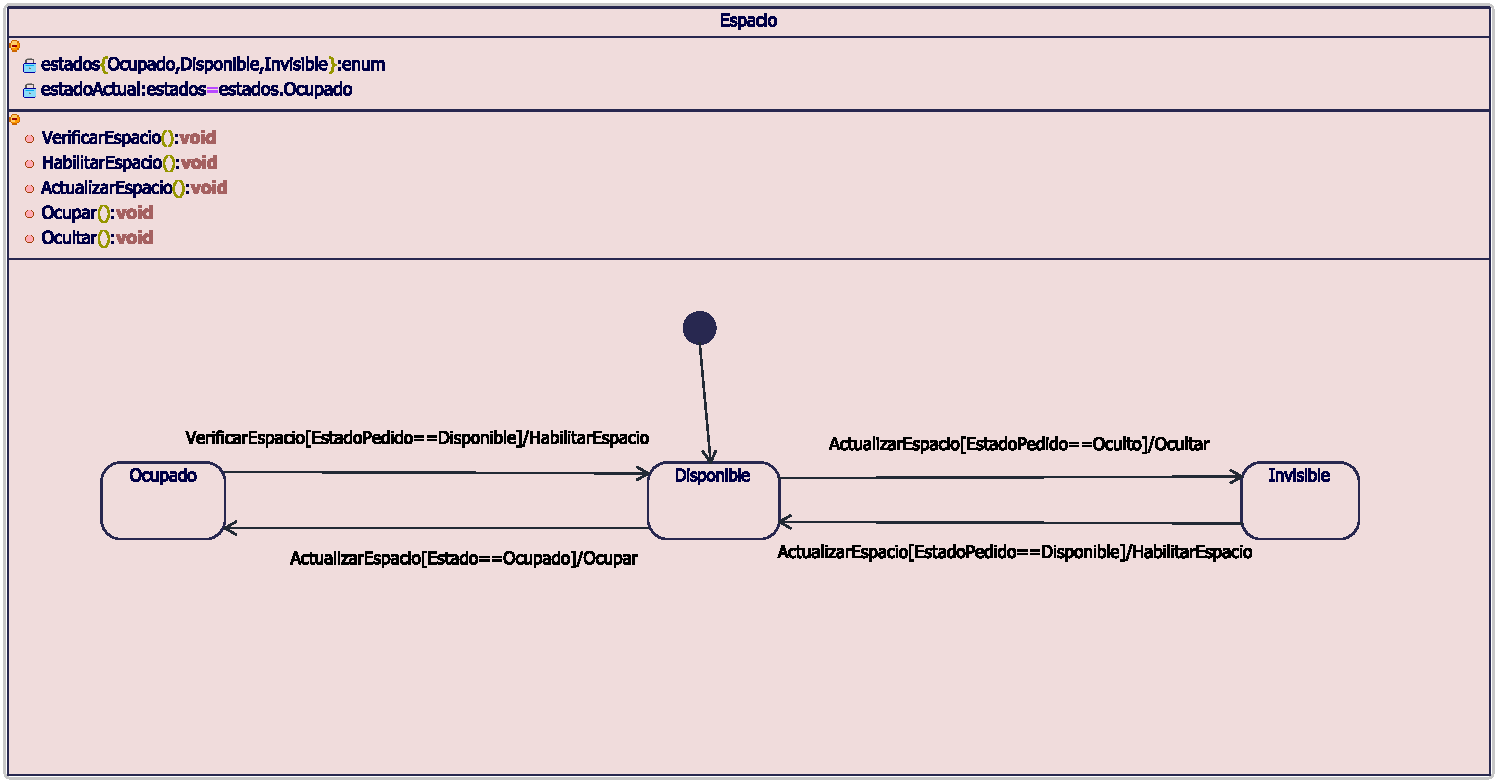
\includegraphics[width=1.18\linewidth]{imgs/Imagenes - Diagrama de estados/ClaseEstados1}}\end{center}
\end{flushleft}
\newpage
\subsection{Diagrama de Clase: Patron Estado}
\begin{flushleft}
Para una mejor conceptualizacion de lo que representa nuestro diagrama de estados, se diseño un diagrama de clase con el patron Estados, que posee una clase "contexto", que es la que requiere dichos cambios de estados, y que en nuestro caso es la clase "Parqueadero", una clase abstracta "Estados" que representa la entidad que maneja los estados, con sus respectivos metodos y atributos, correspondientes al diagrama anterior, y por ultimo, los tres estados que se van a manejar y que son nuestros "Estados concretos", que heredan los metodos de la clase Estados.
\begin{center}
	{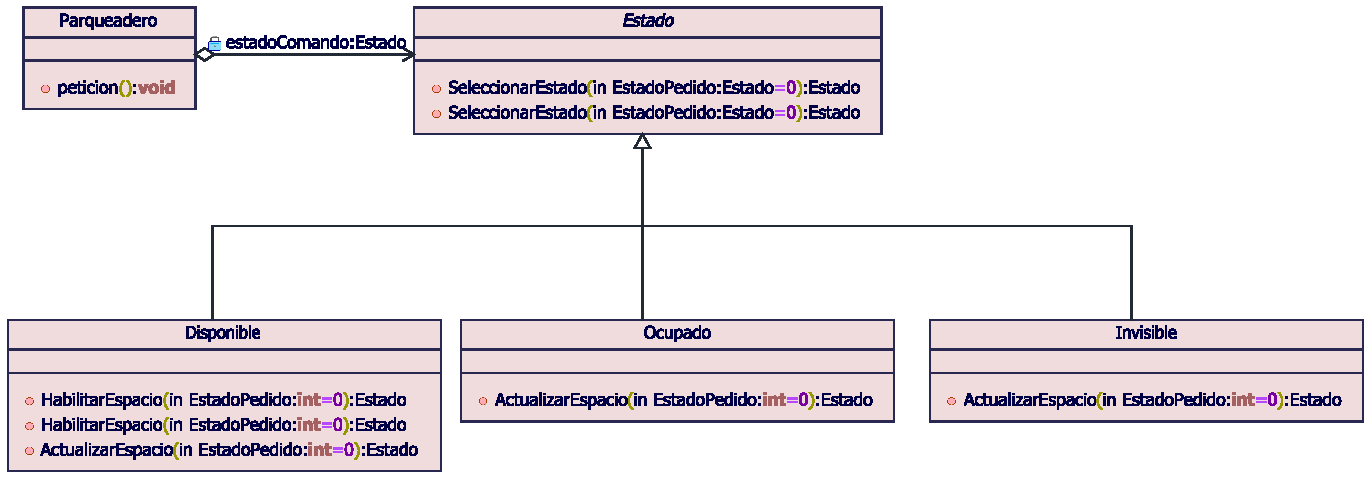
\includegraphics[width=1.18\linewidth]{imgs/Imagenes - Diagrama de estados/ClaseEstados3}}\end{center}
\end{flushleft}

\newpage
\subsection{Diagrama de Secuencia}
\begin{flushleft}
	Por ultimo, para realizar nuestros cambios de estados de una manera concreta, y sin cometer errores, se deben seguir una serie de pasos en el programa, por lo tanto, se diseño el siguiente diagrama de secuencia que representa la serie de pasos que debe seguir el programa para ir de un estado a otro, ademas, como se puede apreciar en el diagrama de estados, no todos los estados estan conectados por una transicion, es decir, no se puede pasar de un estado a otro arbitrariamente, esto se puede ver tambien en el diagrama de secuencia:
	\begin{center}
		{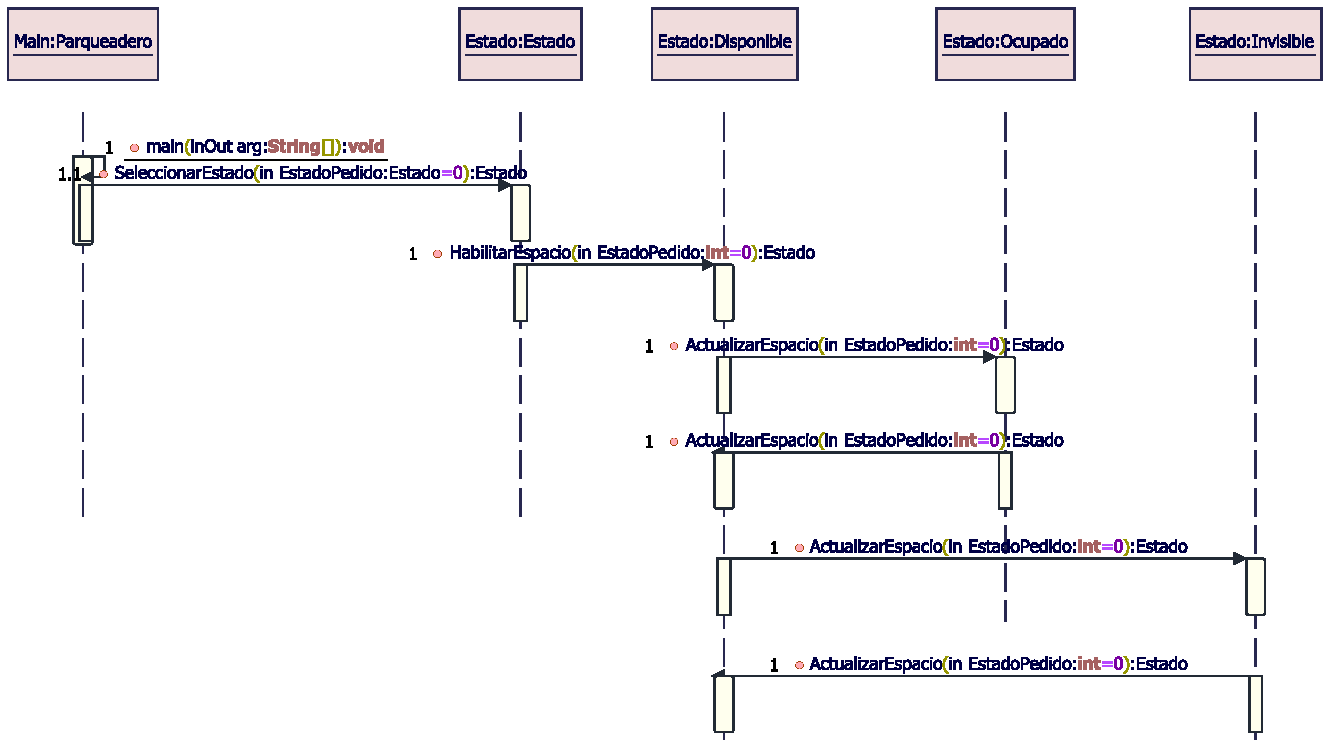
\includegraphics[width=1.18\linewidth]{imgs/Imagenes - Diagrama de estados/SecuenciaEstados}}\end{center}
\end{flushleft}
\newpage
\section{Anexo 1:}
\begin{flushleft}
	Una persona puede tener varios estados de animo en general, pero solo puede tener uno a la vez, es decir, debe haber un cambio de estado en la persona cada vez que quiera experimentar uno diferente.\\
	Para ver un ejemplo de lo anterior enfocado a la Ingenieria de Sofware, se creo el siguiente diagrama de estados de una persona con 3 estados de animo:
	\begin{center}
		{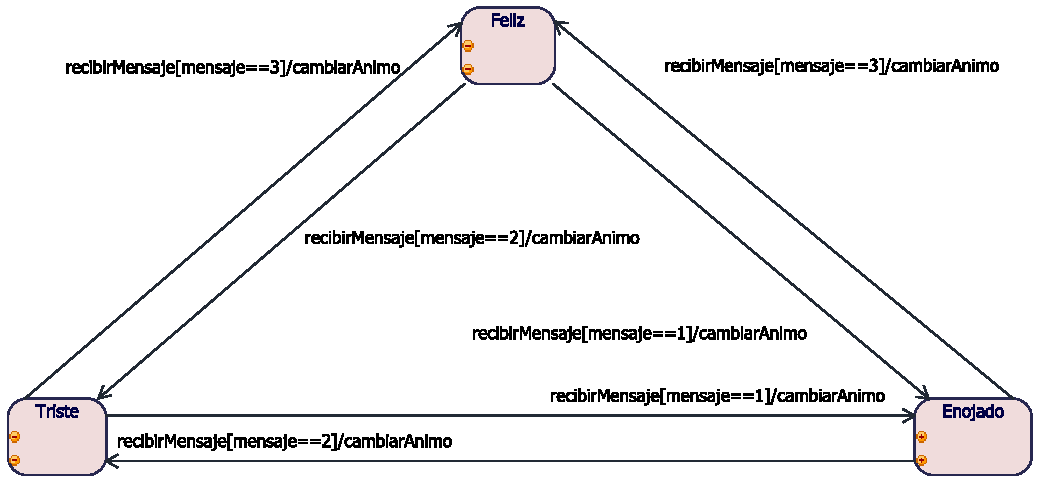
\includegraphics[width=1.18\linewidth]{imgs/Imagenes - Diagrama de estados/Anexo 1/estadosAnimo}}\end{center}
\end{flushleft}

\newpage
\subsection{Anexo 1: Diagrama de clase}
Este diagrama de estados con su respectivo diagrama de clases, con sus metodos y atributos correspondientes:
\begin{center}
	{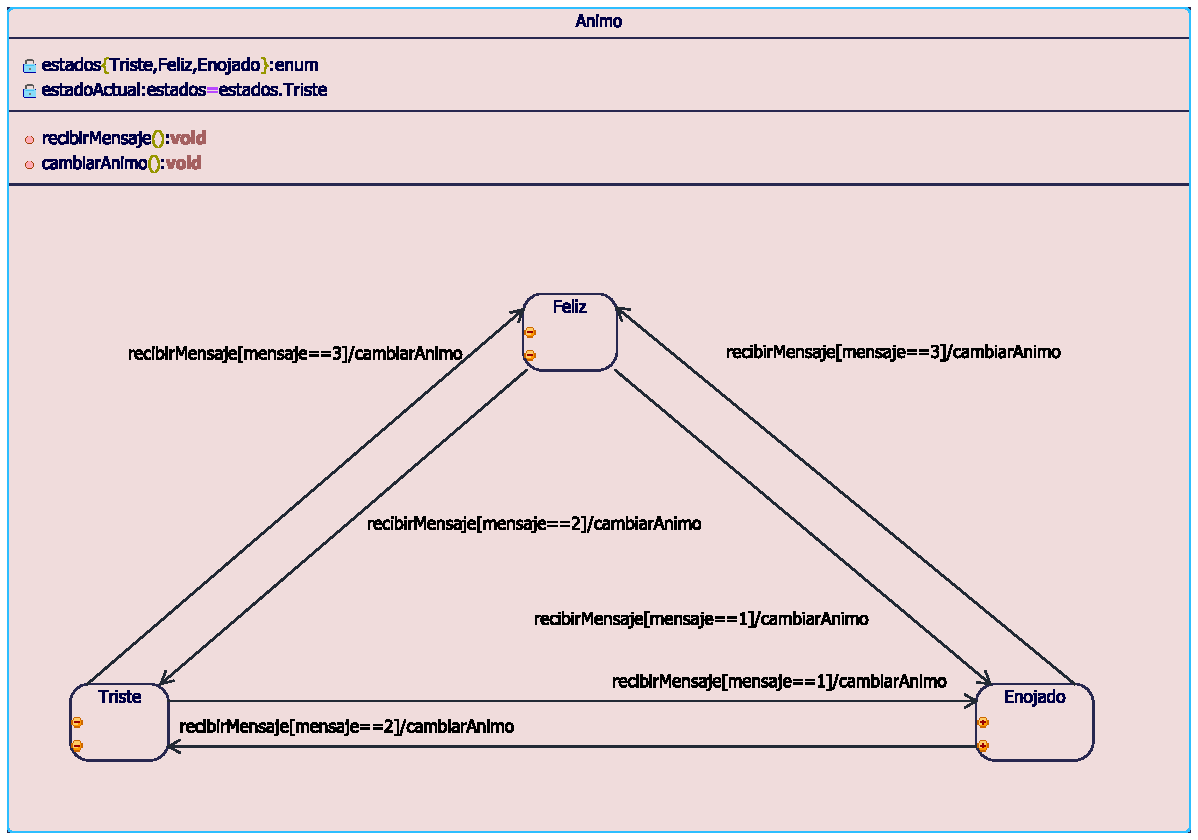
\includegraphics[width=1.18\linewidth]{imgs/Imagenes - Diagrama de estados/Anexo 1/animoclases}}\end{center}
\newpage
\subsection{Anexo 1: Diagrama de Clase del Patrón Estado}
\begin{flushleft}
	El patron Estado nos ayuda a entender mejor el funcionamiento de un diagrama de estados, nosotros hemos diseñado uno para el ejemplo de los estados de animo de una persona:
	\begin{center}
		{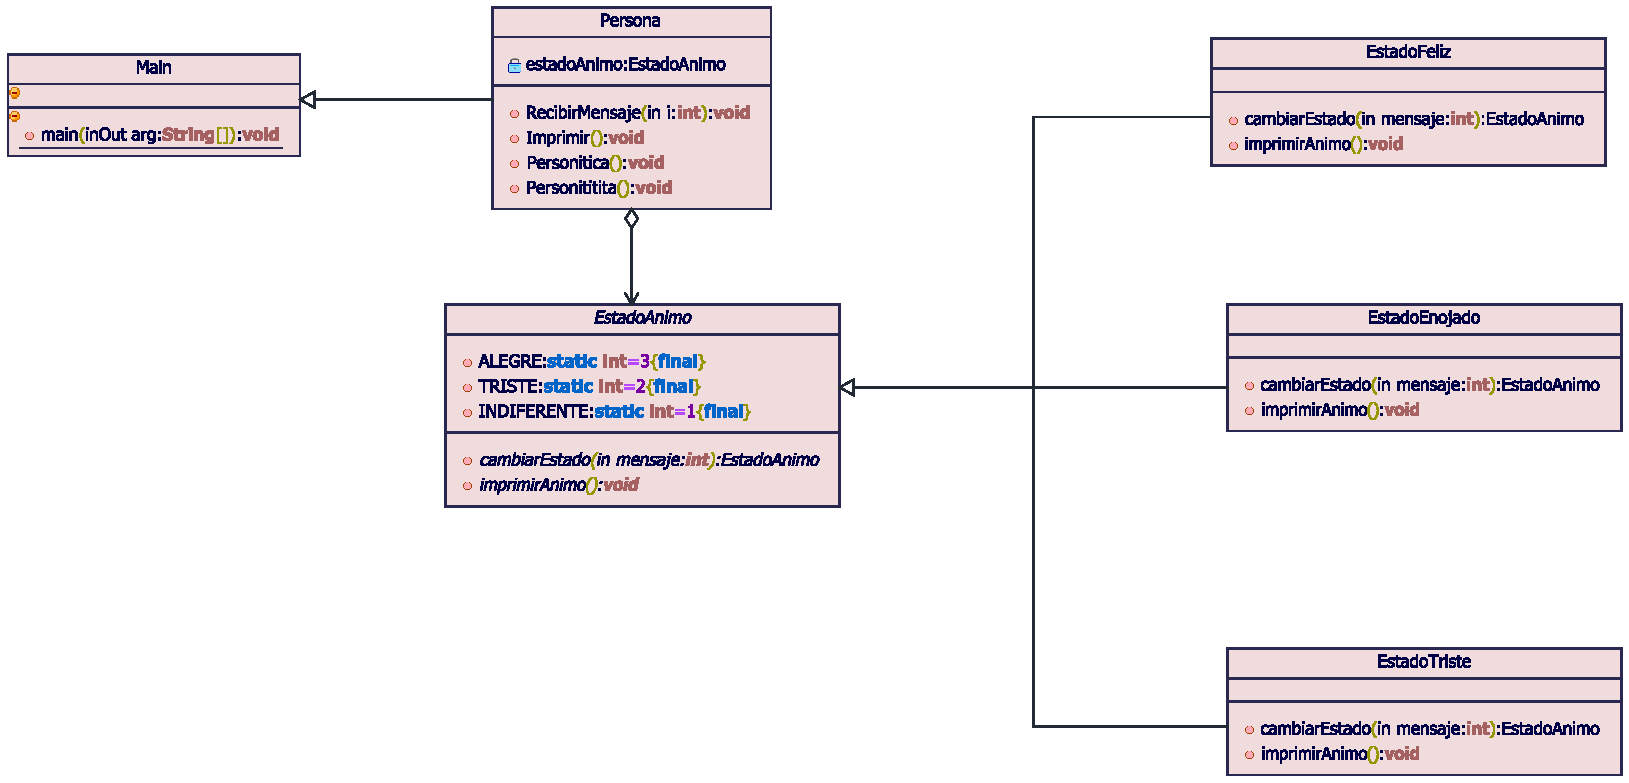
\includegraphics[width=1.18\linewidth]{imgs/Imagenes - Diagrama de estados/Anexo 1/diagramapatrones}}\end{center}
\end{flushleft}
\newpage
\subsection{Anexo 1: Diagrama de Secuencia Extendido}
\begin{flushleft}
	Una vez ponemos a prueba lo aprendido, y partiendo de nuestro diagrama de clase del Patron Estado, hemos construido un diagrama de secuencia extendido en la herramienta de diseño y programacion Coloso, donde es posible ejecutar dicho diagrama de secuencia, que principalmente es el diseño de un software que varia los estados de animo de una persona, entre triste, feliz y enojado, tal y como se ha visto en los anteriores diagramas:
	\begin{center}
		{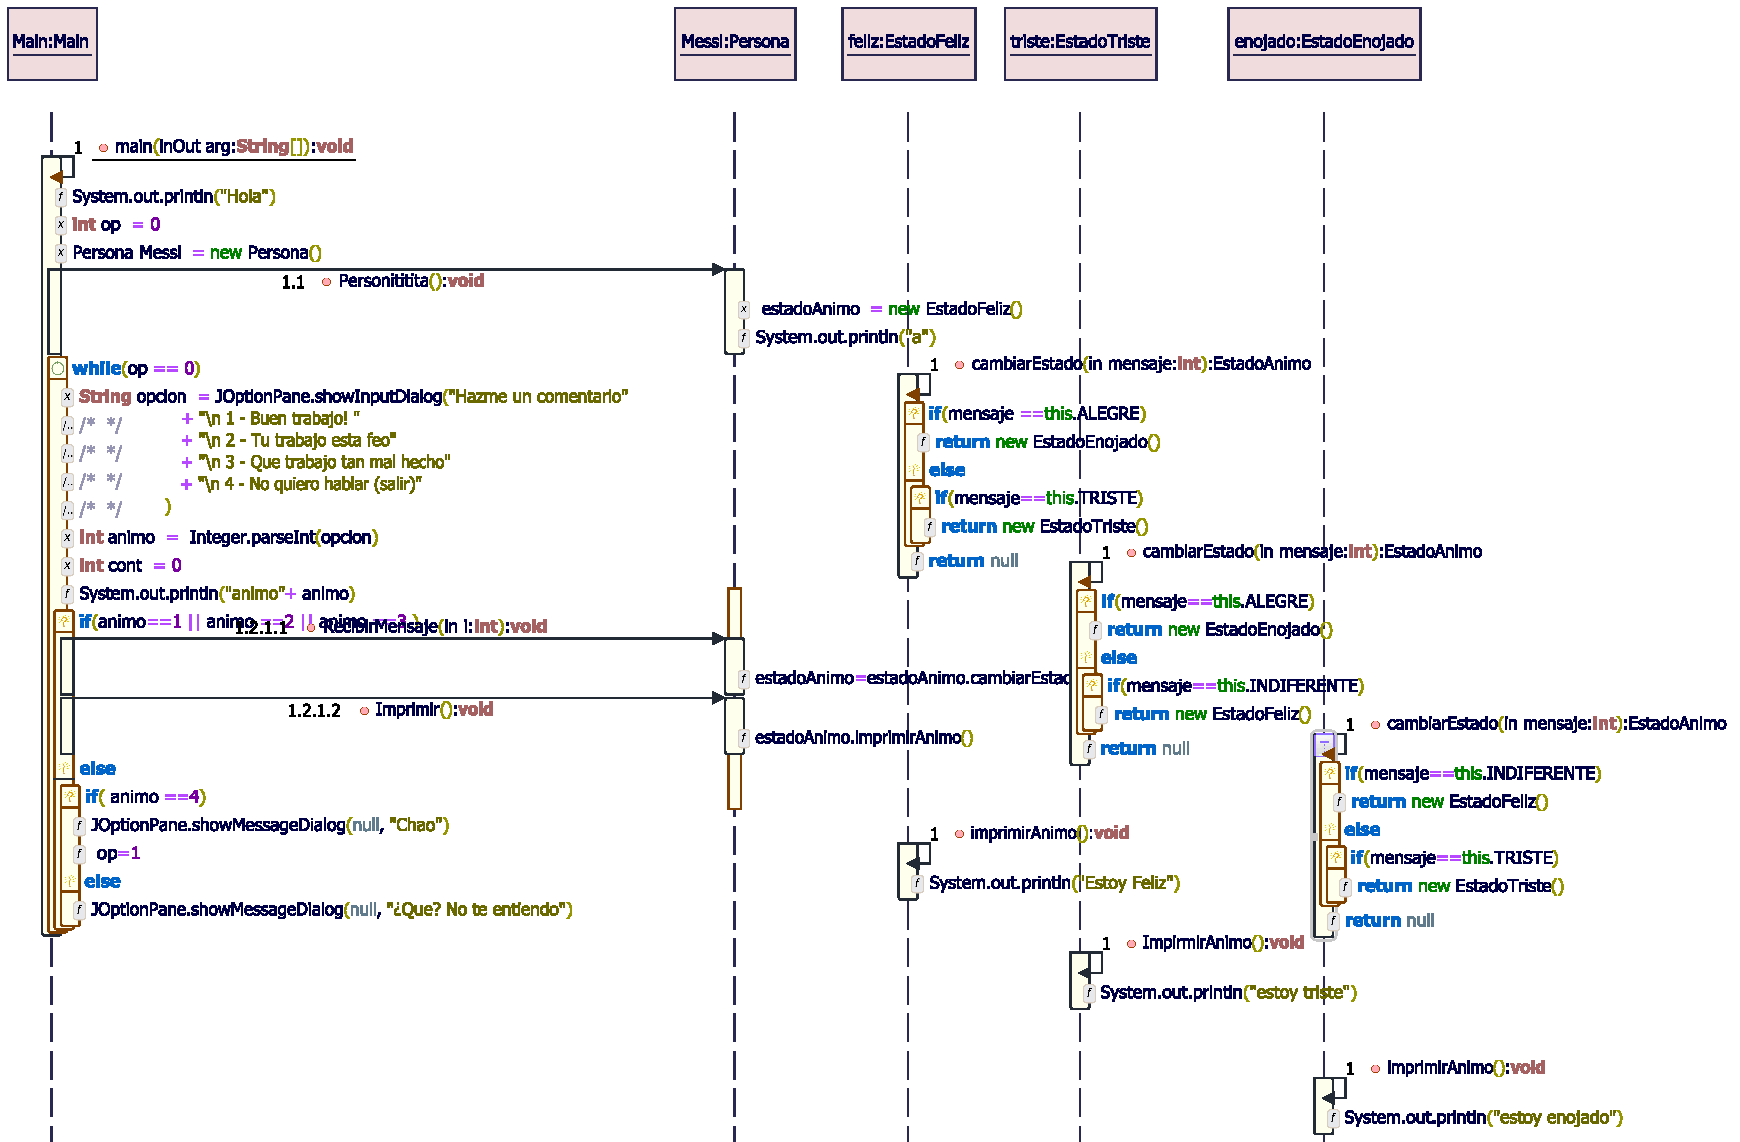
\includegraphics[width=1.28\linewidth]{imgs/Imagenes - Diagrama de estados/Anexo 1/diagramasecuencia}}\end{center}
\end{flushleft}

